
%%%%%%%%%%%%%%%%%%%%%%%%%%%%%%%%%%%%%%%%%%%%%%%%%%%%%%%%%%%
\section{Experiment}\label{sec:expResults}
%%%%%%%%%%%%%%%%%%%%%%%%%%%%%%%%%%%%%%%%%%%%%%%%%%%%%%%%%%%



\subsection{Hardware system}


Our experiments are on centimeter-scale hardware systems.  It allows us to emulate a variety of dynamics, while enabling a high degree of control over robot function, the environment, and data collection. The kilobot \cite{Rubenstein2012,rubenstein2014programmable} is a low-cost robot designed for testing collective algorithms with large numbers of robots. It is available commercially or as an open source platform~\cite{K-Team2015}.  Each robot is approximately 3 cm in diameter, 3 cm tall, and uses two vibration motors to move on a flat surface at speeds up to 1 cm/s.  Each robot has one ambient light sensor that is used to implement \emph{phototaxis},  moving towards a light source. 
In these experiments as shown in Fig.~\ref{fig:setup} , we used $n$=68 kilobots, a 1.5 m$\times$1.2 m whiteboard as the workspace, and four 30W LED floodlights arranged at the $\{N,E,S,W\}$ vertices of a 6 m square centered on the workspace. The lights were controlled by using an Arduino Uno board connected to an 8 relay shield board. Also at top of the table, an overhead machine vision system was added to track the position of the swarm.

\begin{figure}
\begin{center}
	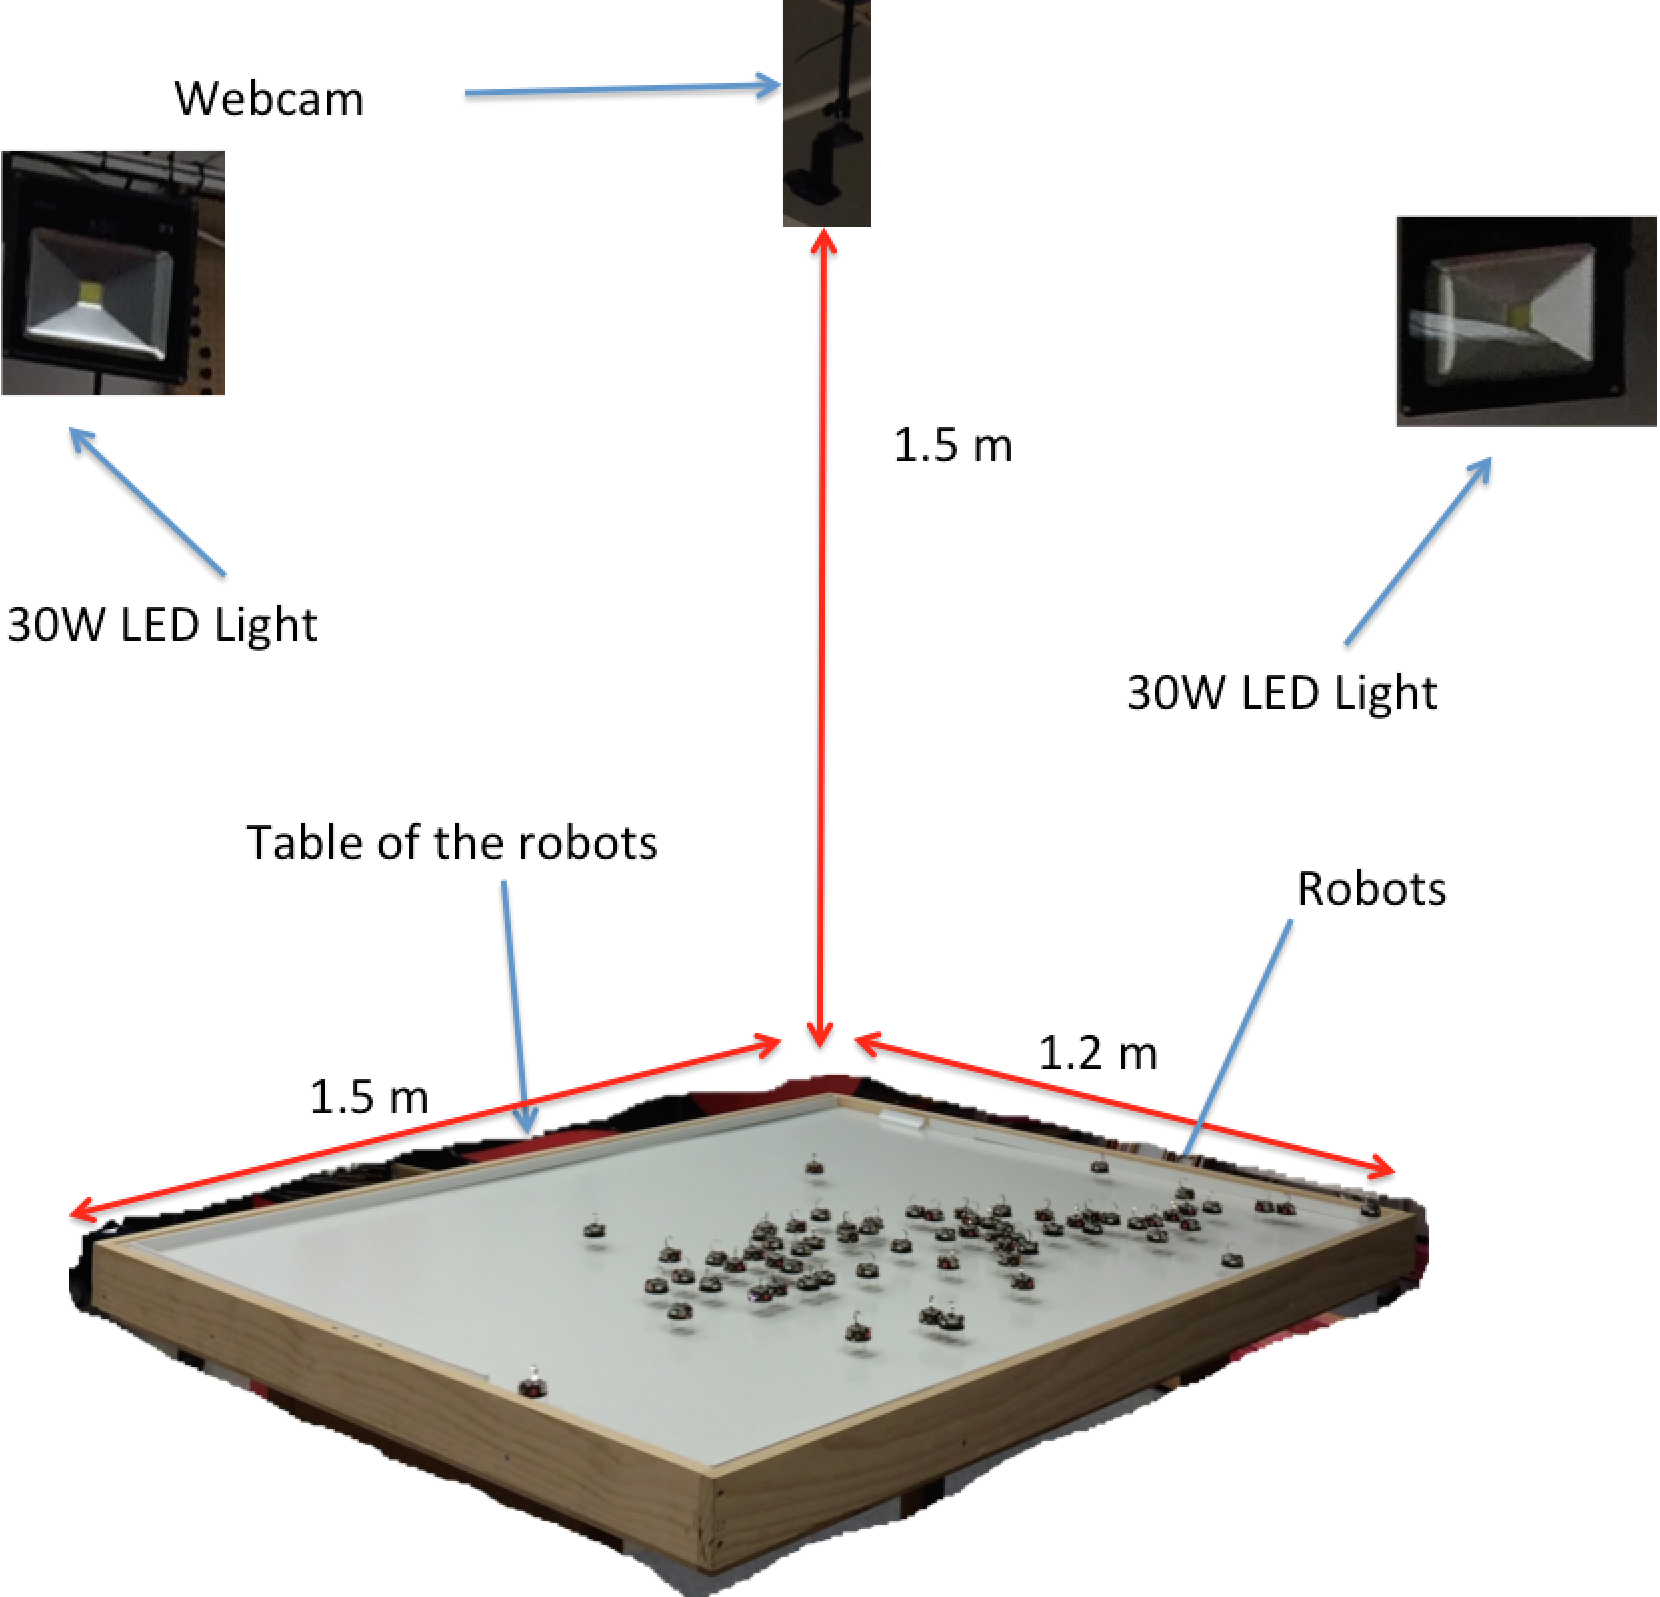
\includegraphics[width=\columnwidth*2/3]{SetUp.png}
\end{center}
\caption{\label{fig:setup}
Our workspace with a table of 1.5$\times$1.2 m and four 30W LED floodlights and an overhead machine vision system.
}
\end{figure}